\documentclass{beamer}
\usepackage{up}

\title{Основни елементи на C++}

\date{5 октомври 2016 г.}

\begin{document}

\begin{frame}
  \titlepage
\end{frame}

\begin{frame}
  \frametitle{Азбука}
  \begin{center}
    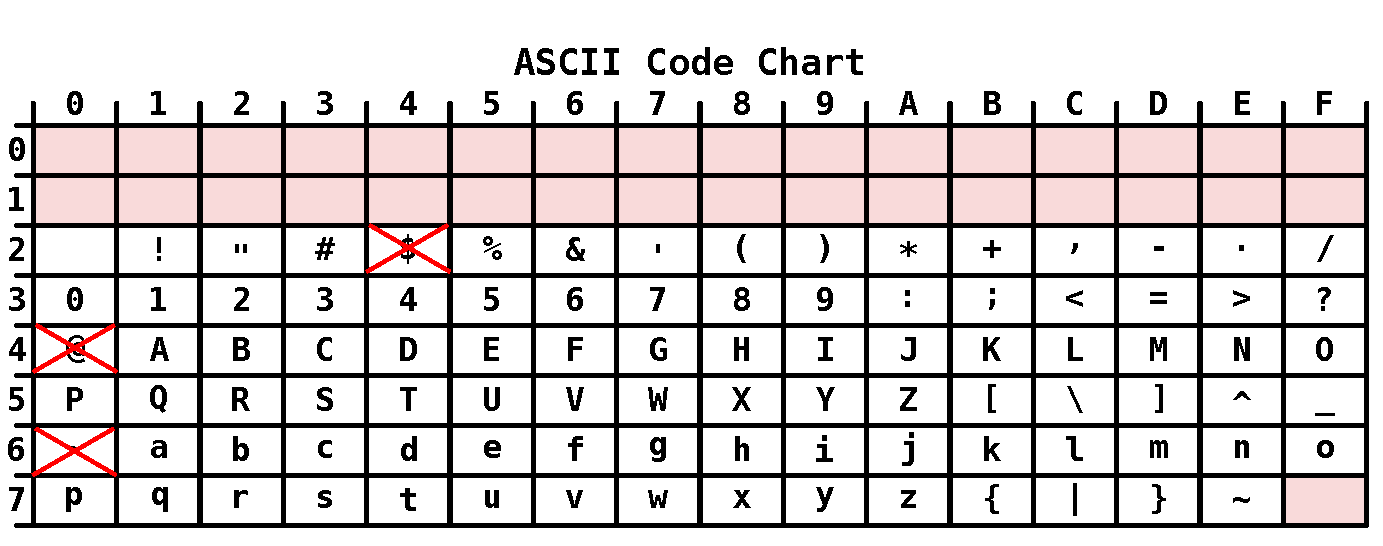
\includegraphics[width=0.9\textwidth]{images/ascii.pdf}\\[2em]
  \end{center}
  \wiki
\end{frame}

\begin{frame}
  \frametitle{Синтаксис}
  \begin{itemize}[<+->]
  \item Правила за построяване на текст
  \item \alert{Иван чете интересна книга.}
  \item \alert{Студентът пише програма.}
  \item \alert{книга. чете Иван? интерес на}
  \item\ <изречение> ::= <подлог> <сказуемо> [ <определение> ] <допълнение>\alert.
  \item\ <подлог> ::= <собствено\_съществително> | <нарицателно\_съществително><пълен\_член>
  \item\ <пълен\_член> ::= \alert{ът} | \alert{ят} | \alert{та} | \alert{то}
  \item\ <сказуемо> ::= <глагол>
  \item\ <определение> ::= <прилагателно>
  \item\ <допълнение> ::= <собствено\_съществително> | <нарицателно\_съществително>
  \end{itemize}
\end{frame}

\begin{frame}
  \frametitle{Синтактичен анализ — пример 1}
  \begin{itemize}[<+->]
  \item\ <изречение>
  \item\ <подлог> <сказуемо> [ <определение> ] <допълнение>\alert.
  \item\ <собствено\_съществително> <сказуемо> <определение> <допълнение>\alert.
  \item \alert{Иван} <глагол> <определение> <допълнение>\alert.
  \item \alert{Иван чете} <определение> <нарицателно\_съществително>\alert.
  \item \alert{Иван чете} <прилагателно> \alert{книга.}
  \item \alert{Иван чете интересна книга.}
  \end{itemize}
\end{frame}

\begin{frame}
  \frametitle{Синтактичен анализ — пример 2}
  \begin{itemize}[<+->]
  \item\ <изречение>
  \item\ <подлог> <сказуемо> [ <определение> ] <допълнение>\alert.
  \item\ <нарицателно\_съществително><пълен\_член> <сказуемо> <допълнение>\alert.
  \item \alert{Студент}{}<пълен\_член> <глагол> <допълнение>\alert.
  \item \alert{Студентът} <глагол> <нарицателно\_съществително>\alert.
  \item \alert{Студентът} <глагол> \alert{програма.}
  \item \alert{Студентът пише програма.}
  \end{itemize}
\end{frame}

\begin{frame}
  \frametitle{Синтактичен анализ — пример 3}
  \begin{itemize}[<+->]
  \item\ <изречение>
  \item\ <подлог> <сказуемо> [ <определение> ] <допълнение>\alert.
  \item\ <нарицателно\_съществително><пълен\_член> <сказуемо> <собствено\_съществително>\alert.
  \item \alert{Програма}{}<пълен\_член> <глагол> \alert{Иван.}
  \item \alert{Програмата гледа Иван.} \onslide<+-> 
\includegraphics[width=20ex, right]{images/creepy.png}
  \item Освен да е построено правилно, изречението трябва да има смисъл!
  \item \textbf{Семантика:} смисъл, значение на текст
  \end{itemize}
\end{frame}

\begin{frame}
  \frametitle{Мета-език на Backus-Naur}
  \begin{itemize}[<+->]
  \item\ <цифра> ::= \tta0 | \tta1 | \tta2 | \tta3 | \tta4 | \tta5 | \tta6 | \tta7 | \tta8 | \tta9
  \item\ <цяло\_число\_без\_знак> ::= <цифра> \{<цифра>\}
  \item\ <цяло\_число> ::= [\tta{+}|\tta{-}] <цяло\_число\_без\_знак>
    \begin{itemize}
    \item \tta{-15}, \tta{2}, \tta{+412}
    \end{itemize}
  \item\ <латинска\_буква> ::= \tta{A} | \tta{B} | ... | \tta{Y} | \tta{Z} | \tta{a} | \tta{b} | ... | \tta{y} | \tta{z}
  \item\ <идентификатор> ::=  \tta{\_} | <латинска\_буква> \{<латинска\_буква> | <цифра> | \tta{\_} \}
    \begin{itemize}
    \item \tta{a}, \tta{name}, \tta{X1}, \tta{\_Data15}
    \end{itemize}
  \end{itemize}
\end{frame}

\begin{frame}
  \frametitle{Основни думи на C++ (tokens)}
  \begin{itemize}[<+->]
  \item\ <идентификатор> ::= \tta\_ | <латинска\_буква> \{<латинска\_буква> |
      <цифра> | \tta\_ \}
  \item запазени думи
  \item стандартни идентификатори
  \item литерали
    \begin{itemize}
    \item числови (\tt1, \tt{-5}, \tt{+2.34}, \tt{1e-02}, \tt{012}, \tt{0x123})
    \item символни (\tt{'a'}, \tt{'\textbackslash{}t'})
    \item низови (\tt{"hello"}, \tt{"yes!"}) 
    \end{itemize}
  \item операции (\tt+, \tt-, \tt*, \tt/)
  \item разделители (\tt{: ; , ( ) [ ] \{ \} < >})
  \end{itemize}
\end{frame}

\begin{frame}[fragile]
  \frametitle{Коментари}
  \begin{itemize}[<+->]
  \item\ <коментар> ::= \tta{\textbackslash\textbackslash}<текст\_без\_нов\_ред> |  \tta{/*} <текст> \tta{*/}
  \item Компилаторът игнорира:
    \begin{itemize}
    \item коментари
    \item празни символи (интервал, табулация, нов ред)
    \end{itemize}
  \item Пример:
\begin{lstlisting}
int sum = 0; // нулираме сумата
/*
   @\emph{вече сме готови да започнем пресмятането}@
   @\emph{последователно ще натрупваме поредните числа в sum}@
   @\emph{докато не ги изчерпим всичките}@
*/
...
\end{lstlisting}
  \end{itemize}
\end{frame}

\end{document}
